\documentclass[tikz,border=2mm]{standalone}
\begin{document}
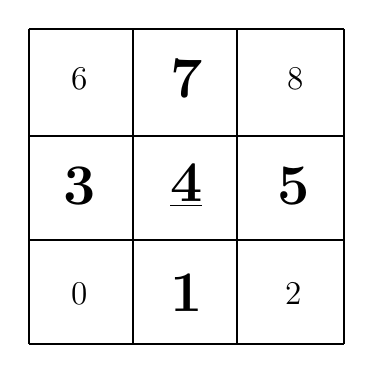
\begin{tikzpicture}[scale=4,thick]
\draw[-] (0,0)--(0,0.33);
\draw[-] (0,0.33)--(0,0.66);
\draw[-] (0,0.66)--(0,1);
\draw[-] (0.33,0)--(0.33,0.33);
\draw[-] (0.33,0.33)--(0.33,0.66);
\draw[-] (0.33,0.66)--(0.33,1);
\draw[-] (0.66,0)--(0.66,0.33);
\draw[-] (0.66,0.33)--(0.66,0.66);
\draw[-] (0.66,0.66)--(0.66,1);
\draw[-] (1,0)--(1,0.33);
\draw[-] (1,0.33)--(1,0.66);
\draw[-] (1,0.66)--(1,1);

\draw[-] (0,0)--(0.33,0);
\draw[-] (0.33,0)--(0.66,0);
\draw[-] (0.66,0)--(1,0);
\draw[-] (0,0.33)--(0.33,0.33);
\draw[-] (0.33,0.33)--(0.66,0.33);
\draw[-] (0.66,0.33)--(1,0.33);
\draw[-] (0,0.66)--(0.33,0.66);
\draw[-] (0.33,0.66)--(0.66,0.66);
\draw[-] (0.66,0.66)--(1,0.66);
\draw[-] (0,1)--(0.33,1);
\draw[-] (0.33,1)--(0.66,1);
\draw[-] (0.66,1)--(1,1);

\large
\draw (0.16,0.16) node {0};
\huge
\draw (0.5,0.16) node {\textbf{1}};
\large
\draw (0.84,0.16) node {2};
\huge
\draw (0.16,0.5) node {\textbf{3}};
\draw (0.5,0.5) node {\underline{\textbf{4}}};
\draw (0.84,0.5) node {\textbf{5}};
\large
\draw (0.16,0.84) node {6};
\huge
\draw (0.5,0.84) node {\textbf{7}};
\large
\draw (0.846,0.84) node {8};
\end{tikzpicture}
\end{document}
